%%%%%%%%%%%%%%%%%%%%%%%%%%%%%%%%%%%%%%%%%%%%%%%%%%%%%%%%%%%%%%%
%
% Welcome to writeLaTeX --- just edit your LaTeX on the left,
% and we'll compile it for you on the right. If you give 
% someone the link to this page, they can edit at the same
% time. See the help menu above for more info. Enjoy!
%
%%%%%%%%%%%%%%%%%%%%%%%%%%%%%%%%%%%%%%%%%%%%%%%%%%%%%%%%%%%%%%%

% --------------------------------------------------------------
% This is all preamble stuff that you don't have to worry about.
% Head down to where it says "Start here"
% --------------------------------------------------------------
 
\documentclass[14pt]{article}
 
\usepackage[margin=0.5in]{geometry} 
\usepackage{amsmath,amsthm,amssymb}
\usepackage{graphicx}
\usepackage{subcaption}
\usepackage{hyperref}
\usepackage{color,soul}
\usepackage{caption}
\usepackage{courier}
\usepackage{float}
\usepackage{listings}
\usepackage{xcolor} % for setting colors


\newcommand{\N}{\mathbb{N}}
\newcommand{\Z}{\mathbb{Z}}


\newenvironment{theorem}[2][Theorem]{\begin{trivlist}

  \item[\hskip \labelsep {\bfseries #1}\hskip \labelsep {\bfseries #2.}]}{\end{trivlist}}
\newenvironment{lemma}[2][Lemma]{\begin{trivlist}
\item[\hskip \labelsep {\bfseries #1}\hskip \labelsep {\bfseries #2.}]}{\end{trivlist}}
\newenvironment{exercise}[2][Exercise]{\begin{trivlist}
\item[\hskip \labelsep {\bfseries #1}\hskip \labelsep {\bfseries #2.}]}{\end{trivlist}}
\newenvironment{problem}[2][Problem]{\begin{trivlist}
\item[\hskip \labelsep {\bfseries #1}\hskip \labelsep {\bfseries #2.}]}{\end{trivlist}}
\newenvironment{question}[2][Question]{\begin{trivlist}
\item[\hskip \labelsep {\bfseries #1}\hskip \labelsep {\bfseries #2.}]}{\end{trivlist}}
\newenvironment{corollary}[2][Corollary]{\begin{trivlist}
\item[\hskip \labelsep {\bfseries #1}\hskip \labelsep {\bfseries #2.}]}{\end{trivlist}}

\newenvironment{solution}{\begin{proof}[Solution]}{\end{proof}}
\newenvironment{courier}{\ttfamily}{\par}

% set the default code style
\lstset{
    frame=tb, % draw a frame at the top and bottom of the code block
    tabsize=4, % tab space width
    showstringspaces=false, % don't mark spaces in strings
    numbers=left, % display line numbers on the left
    commentstyle=\color{orange}, % comment color
    keywordstyle=\color{blue}, % keyword color
    stringstyle=\color{red} % string color
}

\begin{document}
 
% --------------------------------------------------------------
%                         Start here
% --------------------------------------------------------------
 
\title{\textbf{Brief Document On the Hall C Hodoscopes Calibration}}%replace X with the appropriate number
\author{Carlos Yero} %if necessary, replace with your course title
 
\maketitle
\noindent The Hall C Scintillaror Hodoscopes consists on four planes (per spectrometer) of scintillator arrays oriented perpendicular
to the beam direction(See Figure \ref{fig:Hodo}). Each spectrometer has two sets of planes, each set oriented along the +X and +Y in the hut coordinate system.
The hodoscopes form the standard HMS/SHMS trigger in Hall C due to the fast signal rise time produced from the scintillating material.
For a thorough discussion of how the trigger is formed, see . . . \\
\begin{figure}[H]
  \captionsetup{justification=raggedright,singlelinecheck=false}
  \includegraphics[scale=0.3]{Hodo.png}
  \caption{HMS Hodoscope 1X and 1Y Planes.}
  \label{fig:Hodo}
\end{figure}
When a particle traverses a plane, depending on the trajectory, any paddle could in principle be hit,
the paddle then scintillates light, which propagates to them photomultiplier tubes (PMTs) at the two ends. The PMTs
convert the incident light to photoelectrons in the photocathode. The photoelectrons then are guided through the various dynodes in the PMT, knocking
out more electrons, creating an avalanche of electrons. The electron avalanche then reaches the anode, producing a measurable current signal.
The signal is sent to the Counting Room, where it is processed by the NIM/CAMAC electronics, and ultimately sent to ADCs, and TDCs. At this stage, the raw tdc signal
has multiple unwanted timing contributions which must be subtracted to obtain the true arrival time at the hodoscope plane. The corrected tdc time is the used to determine
the correct particle velocity, $\beta = \frac{v}{c}$. The determination and correction for the additional timing from the raw tdc is the essence of the hodoscope timing
calibration, and will be discussed next.

\section{Discussion on the Hodoscope Timing Corrections}
The general expression for the corrected TDC time for a hodoscope PMT is
\begin{equation}
t_{Corr} = t_{RAW} - t_{TW} - t_{Cable} - t_{prop.} - t_{\lambda} 
\end{equation}
\newpage
The corrected TDC time represents the particle arrival time at the scintillator paddle.
The corrections are summarized as follows (See Figure \ref{fig:Paddle}):
\begin{figure}[H]
  \captionsetup{justification=raggedright,singlelinecheck=false}
  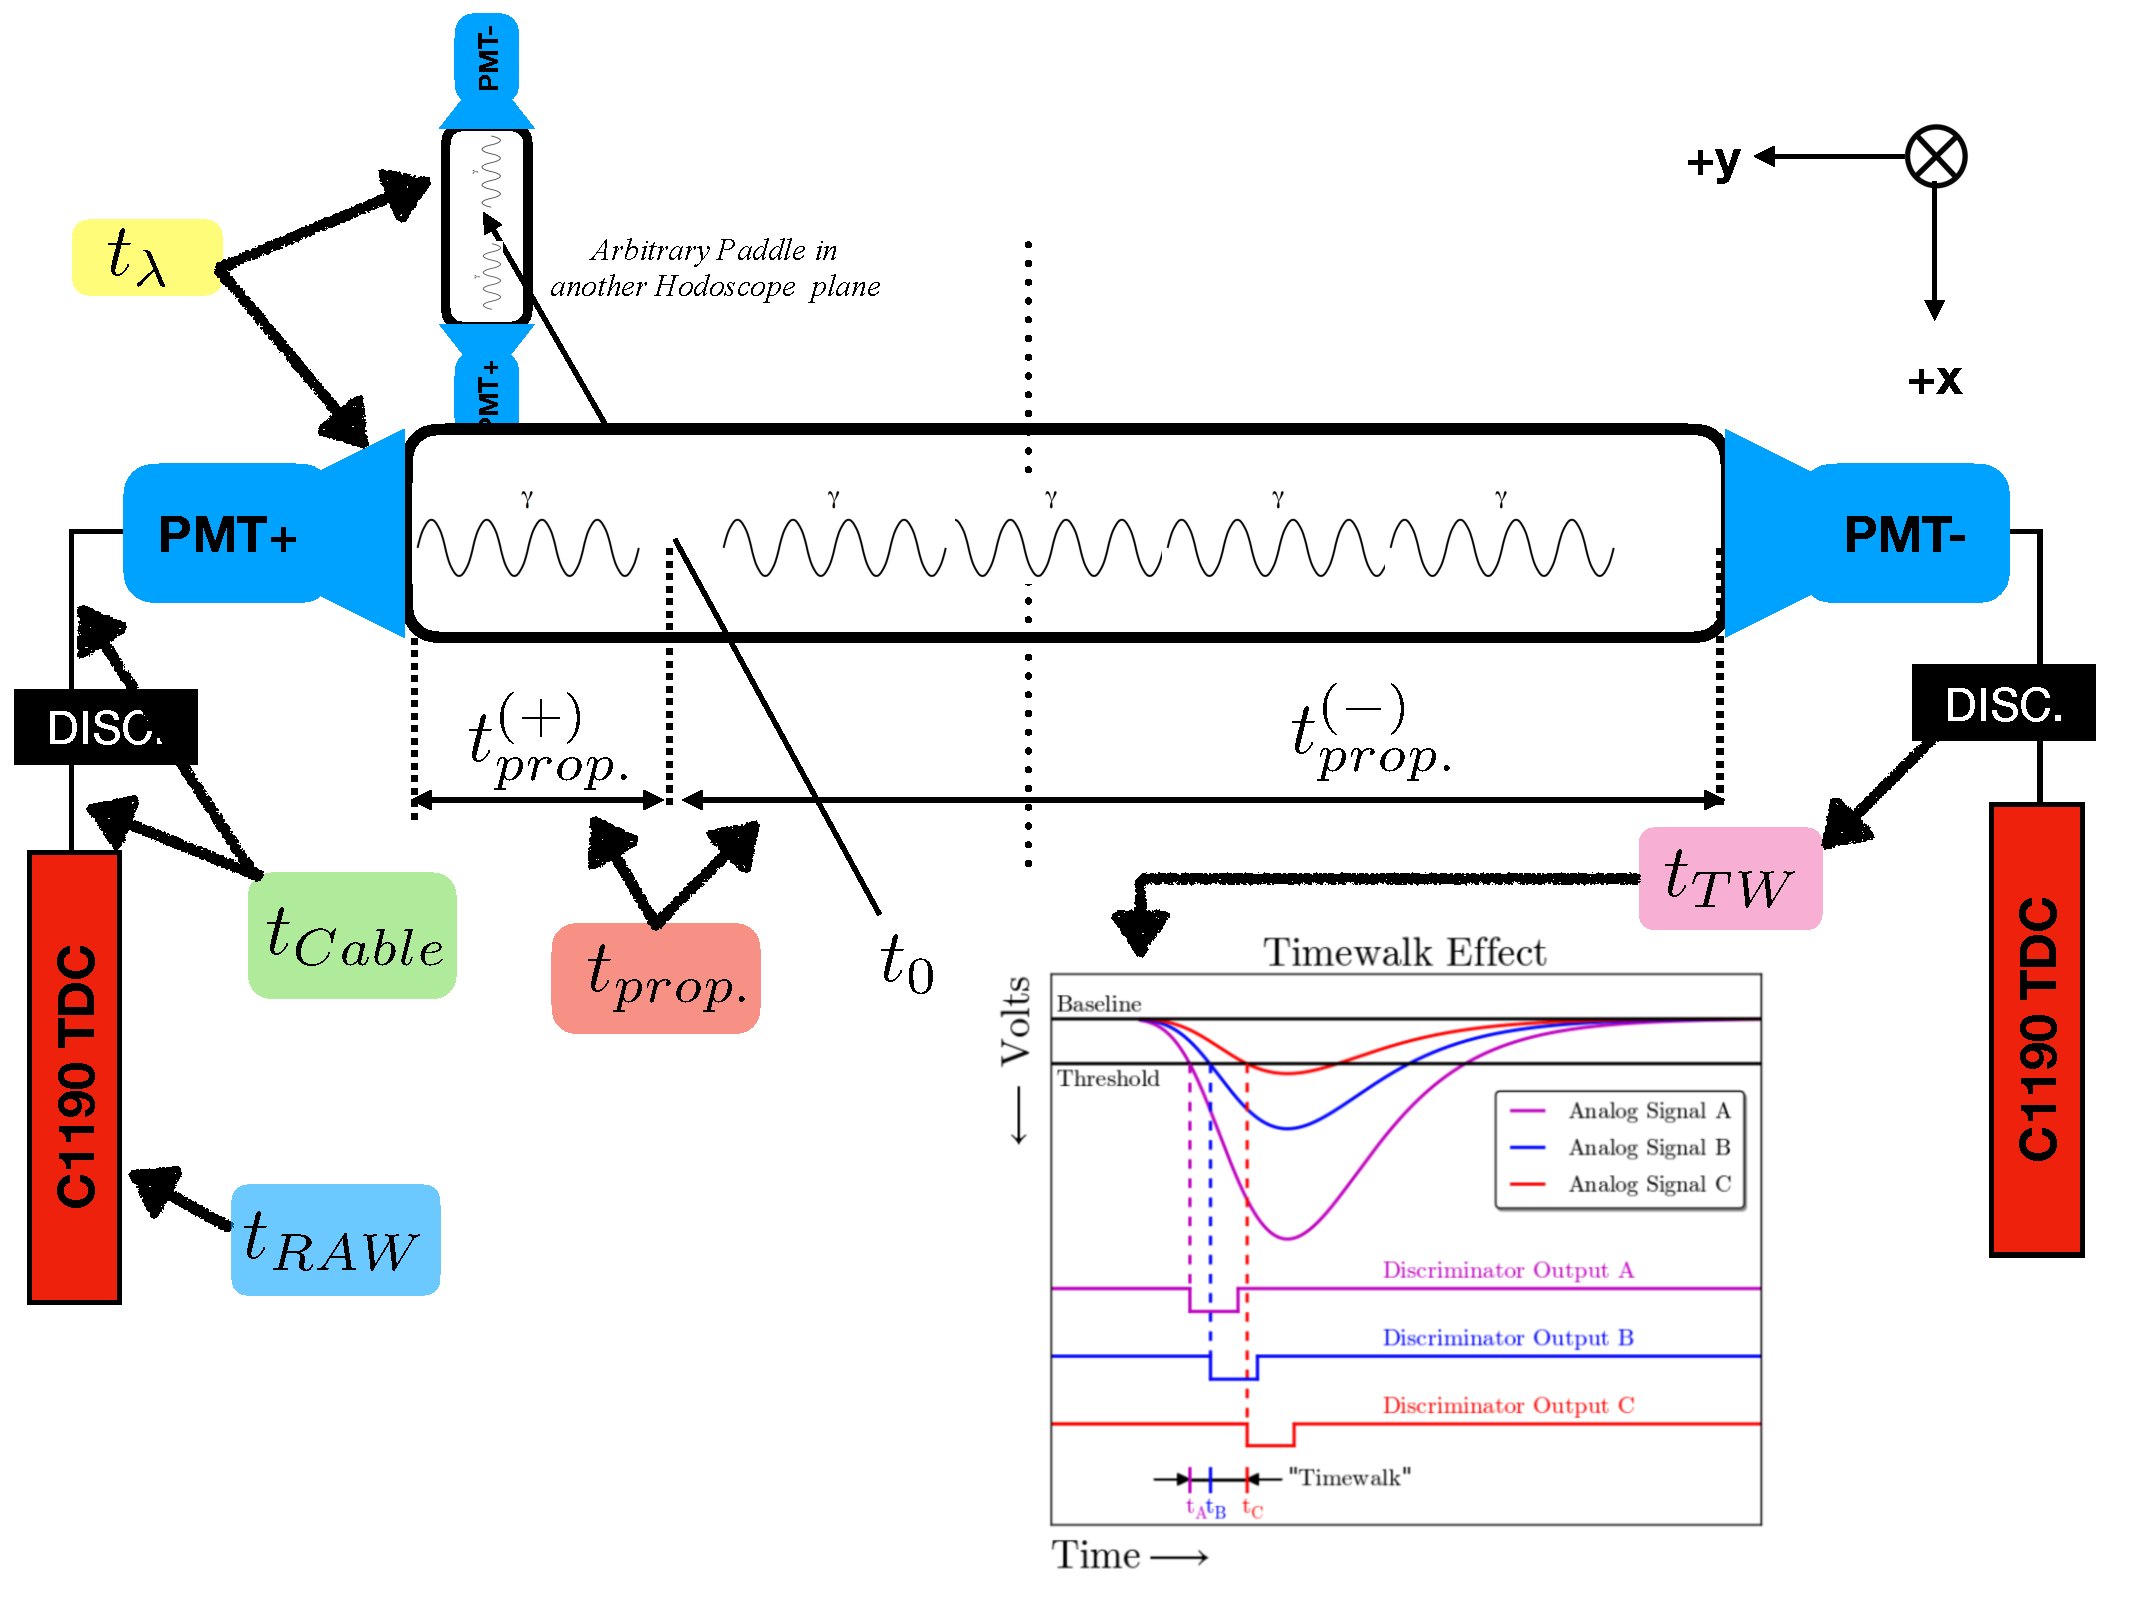
\includegraphics[scale=0.5]{HodoPaddle.pdf}
  \caption{Cartoon of individual scintillator paddles to illustrate the various timing corrections applied.}
  \label{fig:Paddle}
\end{figure}
\begin{itemize}
\item \textbf{Time-Walk Corrections}, $t_{TW}$: For analog signals arriving at the \textit{Leading Edge Discriminators}
  at a particular time, depending on the signal \textit{amplitude}, the leading edge of the signal is discriminated,
  which causes the discriminated logic signal to jitter in time, when it should \textbf{NOT}, since the signals arrived at the
  same time. Analog-to-Digital Converters (ADCs), do not have this disadvantage, since they correct for time-walk internally,
  and as a result, the ADC Pulse Time is not correlated with the signal amplitude. To correct for this correlation in the TDCs,
  the ADC Pulse Time is used as a reference by taking the TDC-ADC Pulse Time difference is plotted against the ADC amplitude. A model
  function is fitted to this correlation, and the parameters extracted are used to correct the TDC time.
\begin{figure}[H]
  \captionsetup{justification=raggedright,singlelinecheck=false}
    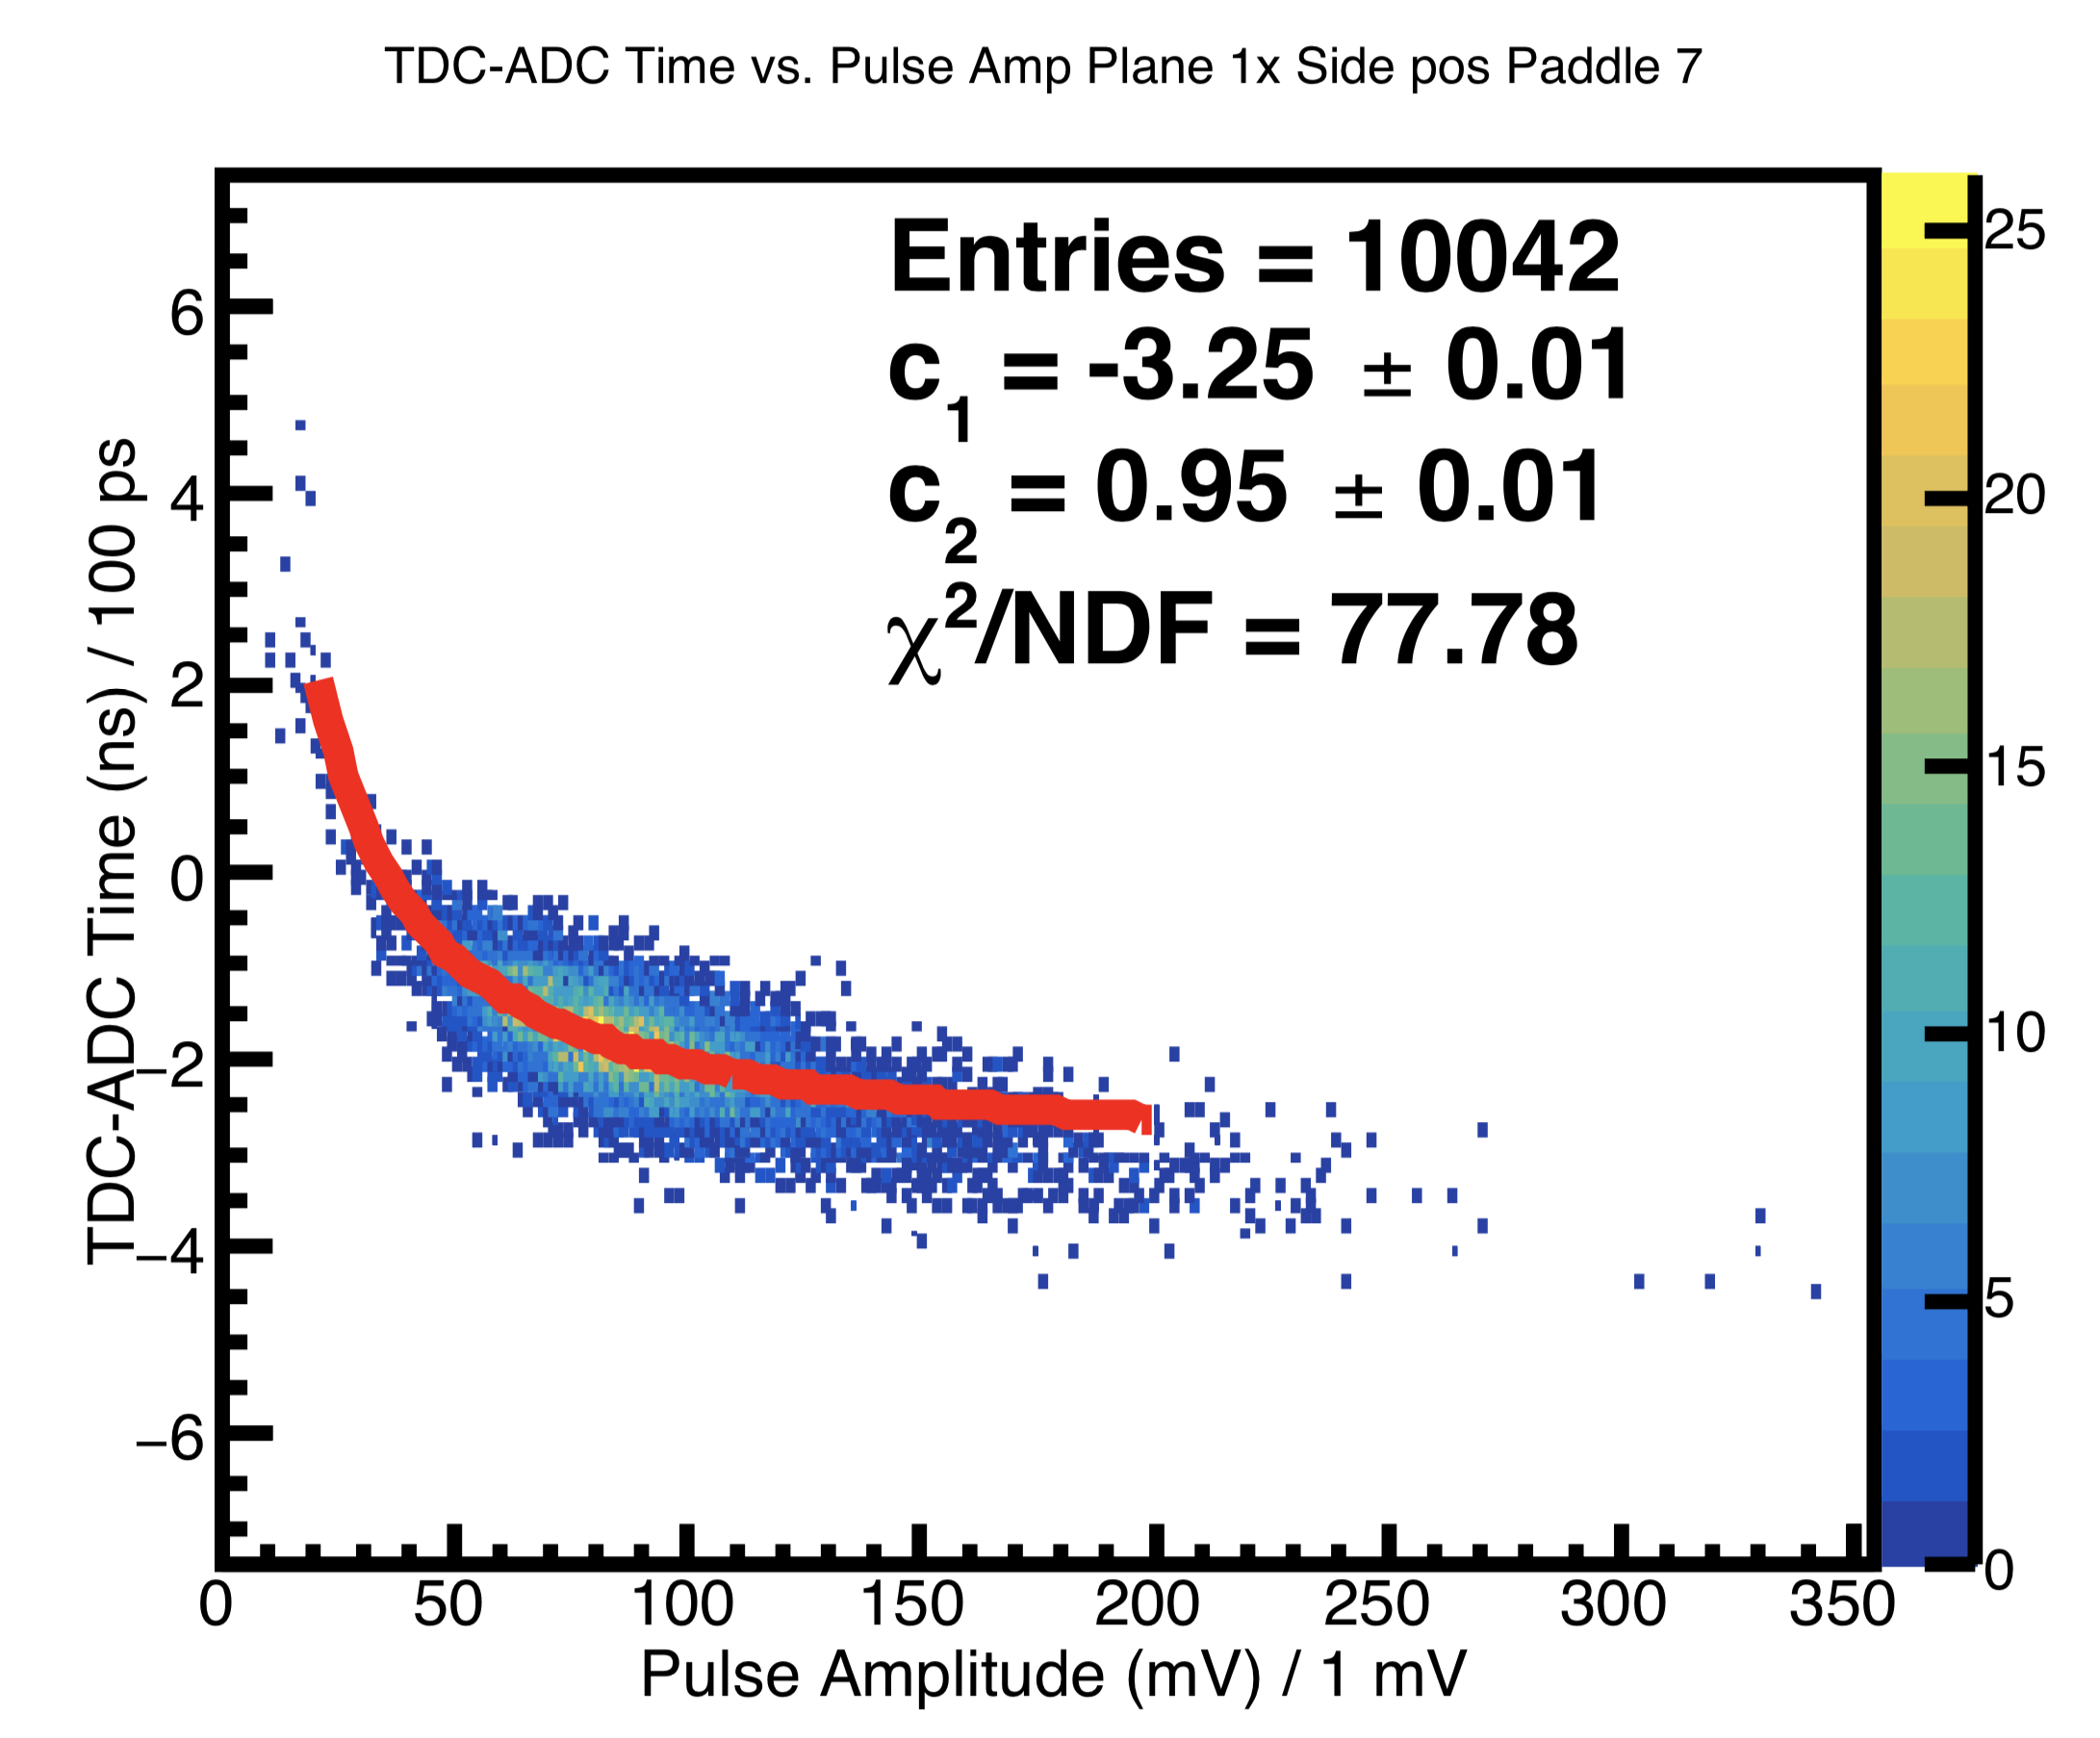
\includegraphics[scale=0.35]{1x7-_TWFit.png}
    \caption{Fitted correlation between TDC pulse Time and ADC Pulse Amplitude.}
    \label{fig:TWFit}
  \end{figure}
\begin{figure}[H]
    \captionsetup{justification=raggedright,singlelinecheck=false}
    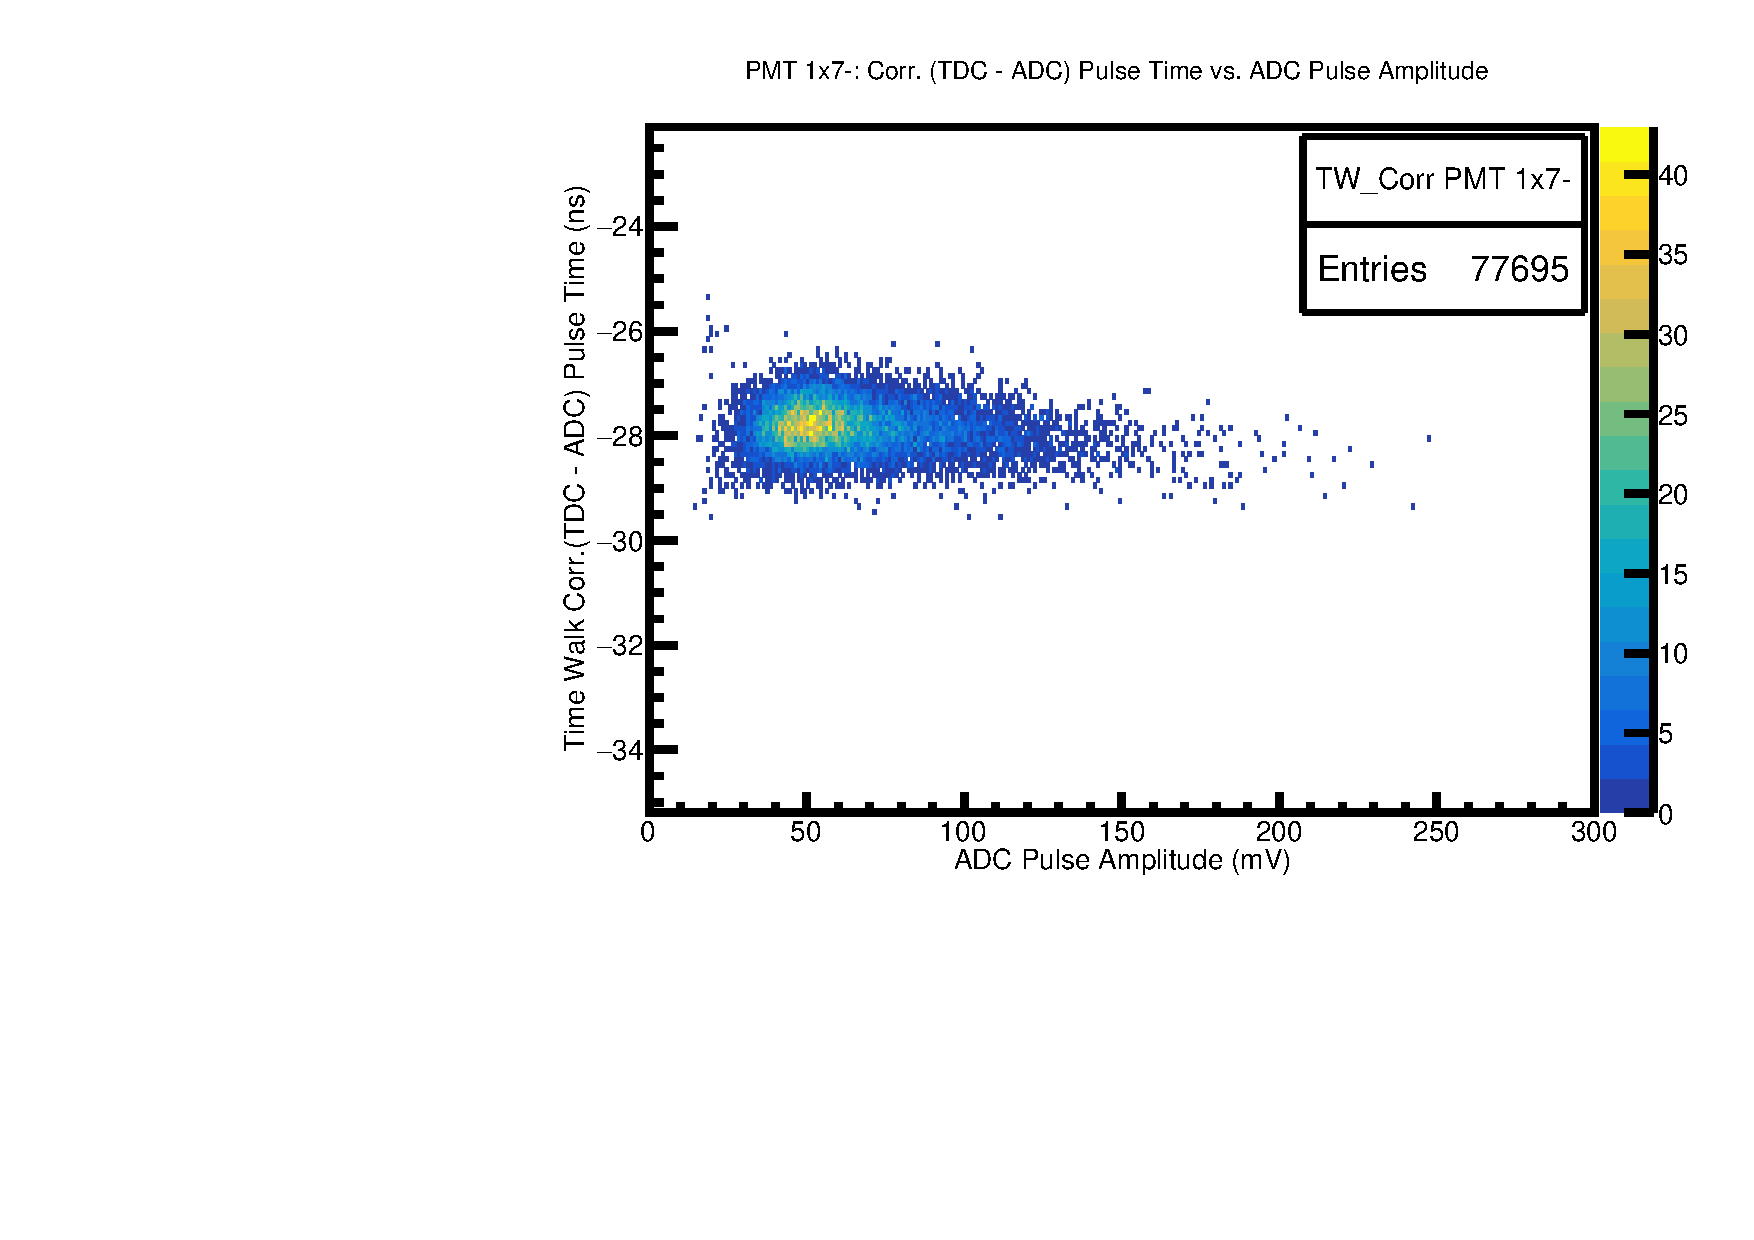
\includegraphics[scale=0.75]{1x7-_TWCorr.pdf}
    \caption{Corrected TDC Time Walk spectrum, where the correlation with Pulse Amplitude has been removed.}
    \label{fig:TWCorr}
  \end{figure}
\newpage
The plot in Figure \ref{fig:TWFit} shows the correlation between TDC Pulse Time and ADC Pulse Amplitude.  The fit parameters, $c_{1}$, TDC Threshold are read in by hcana, where
the time-walk correction is applied to the raw TDC to obtain the corrected tdc time as shown in Figure \ref{fig:TWCorr}.
\item Cable Time Corrections, $t_{Cable}$: This correction takes into account the fact that the analog signal has
  to propagate across signal cables from the PMT all the way into the Counting House electronics rack into the TDC.
  To determine this correction, a correlation between Time-Walk corrected time and hodoscope paddle track position is fitted
  to extract the velocity of propagation across the paddle, and the cable time offset. Figure \ref{fig:Vp} shows the cartoon of a
  horizontal paddle to illustrate how to determine the propagation velocity.
\begin{figure}[H]
    \captionsetup{justification=raggedright,singlelinecheck=false}
    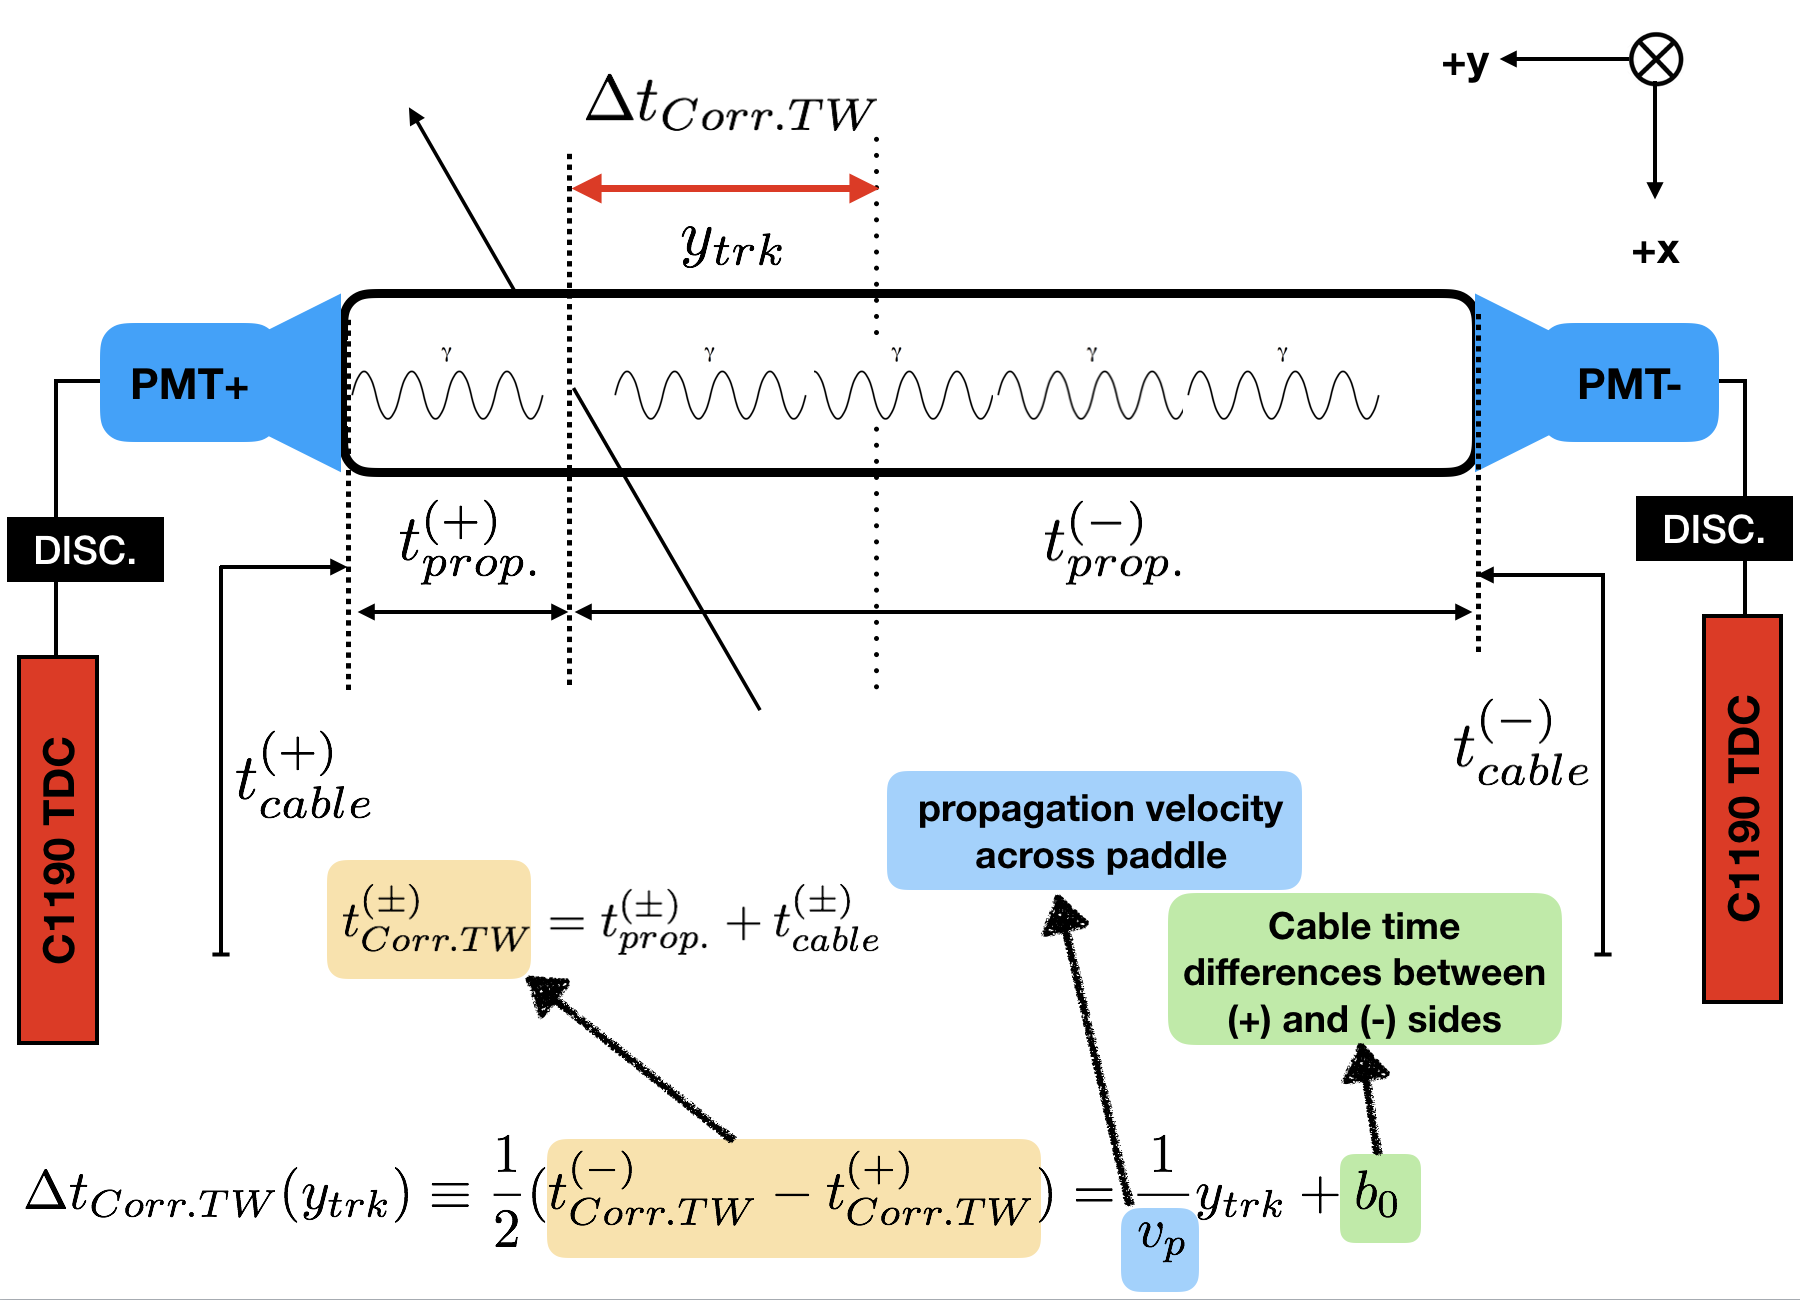
\includegraphics[scale=0.5]{Vp.png}
    \caption{Illustration of how the propagation velocity across a paddle is determined.}
    \label{fig:Vp}
\end{figure}
The propagation velocity is determined from the distance and time of the hit from the center of a paddle.
The time is determined by taking half of the time-walk corrected TDC time difference between the two ends of a paddle.
The \textit{half} is to ensure that if the particle hits the edge of the paddle, half of the total propagation
time across the entire paddle is taken to obtain the time from the edge to the center. The hit distance is
determined by extrapolating the distance determined by the Drift Chambers from tracking. The correlation between
time and distance is fitted to extract the propagation velocity and the cable time difference between the two ends. (See Figure \ref{fig:Vp_fit})
The cable time offset parameter is determined for all paddles and the parameter is read by hcana, and added as a correction
factor to the time-walk corrected TDC time. 
\begin{figure}[H]
    \captionsetup{justification=raggedright,singlelinecheck=false}
    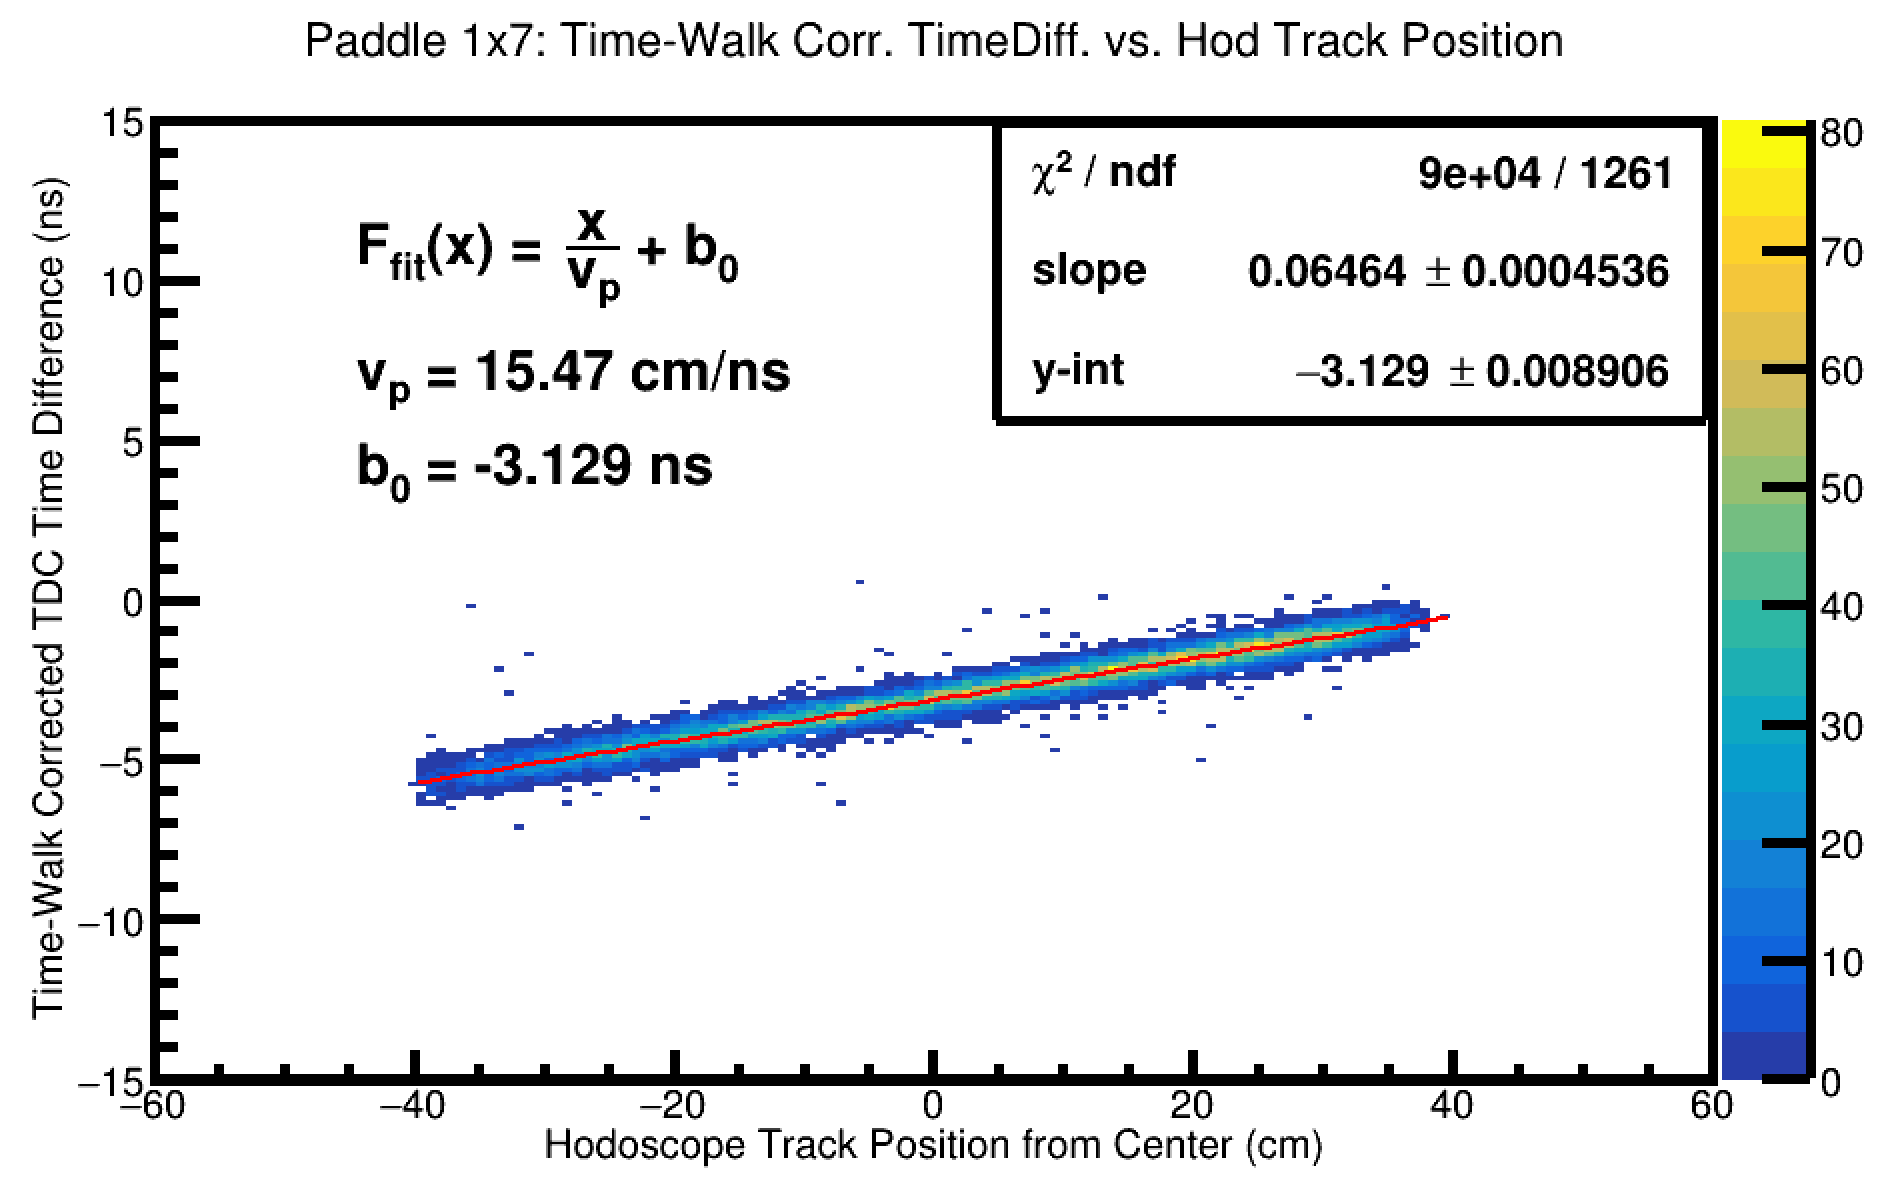
\includegraphics[scale=0.5]{1x7_Velocity.png}
    \caption{Illustration of how the propagation velocity across a paddle is determined.}
    \label{fig:Vp_fit}
\end{figure}
\item Hodoscope Planes Time Difference Corrections, $t_{\lambda}$: This correction accounts for any additional time difference (other than the particle propagation
  time to travel across the two paddles) between any two distinct scintillator paddles in different hodoscope planes. Six possible combinations between
  the four hodoscope planes are considered when correcting for the time difference between any two of their paddles (See Figure \ref{fig:hod_planes})
\begin{figure}[H]
    \captionsetup{justification=raggedright,singlelinecheck=false}
    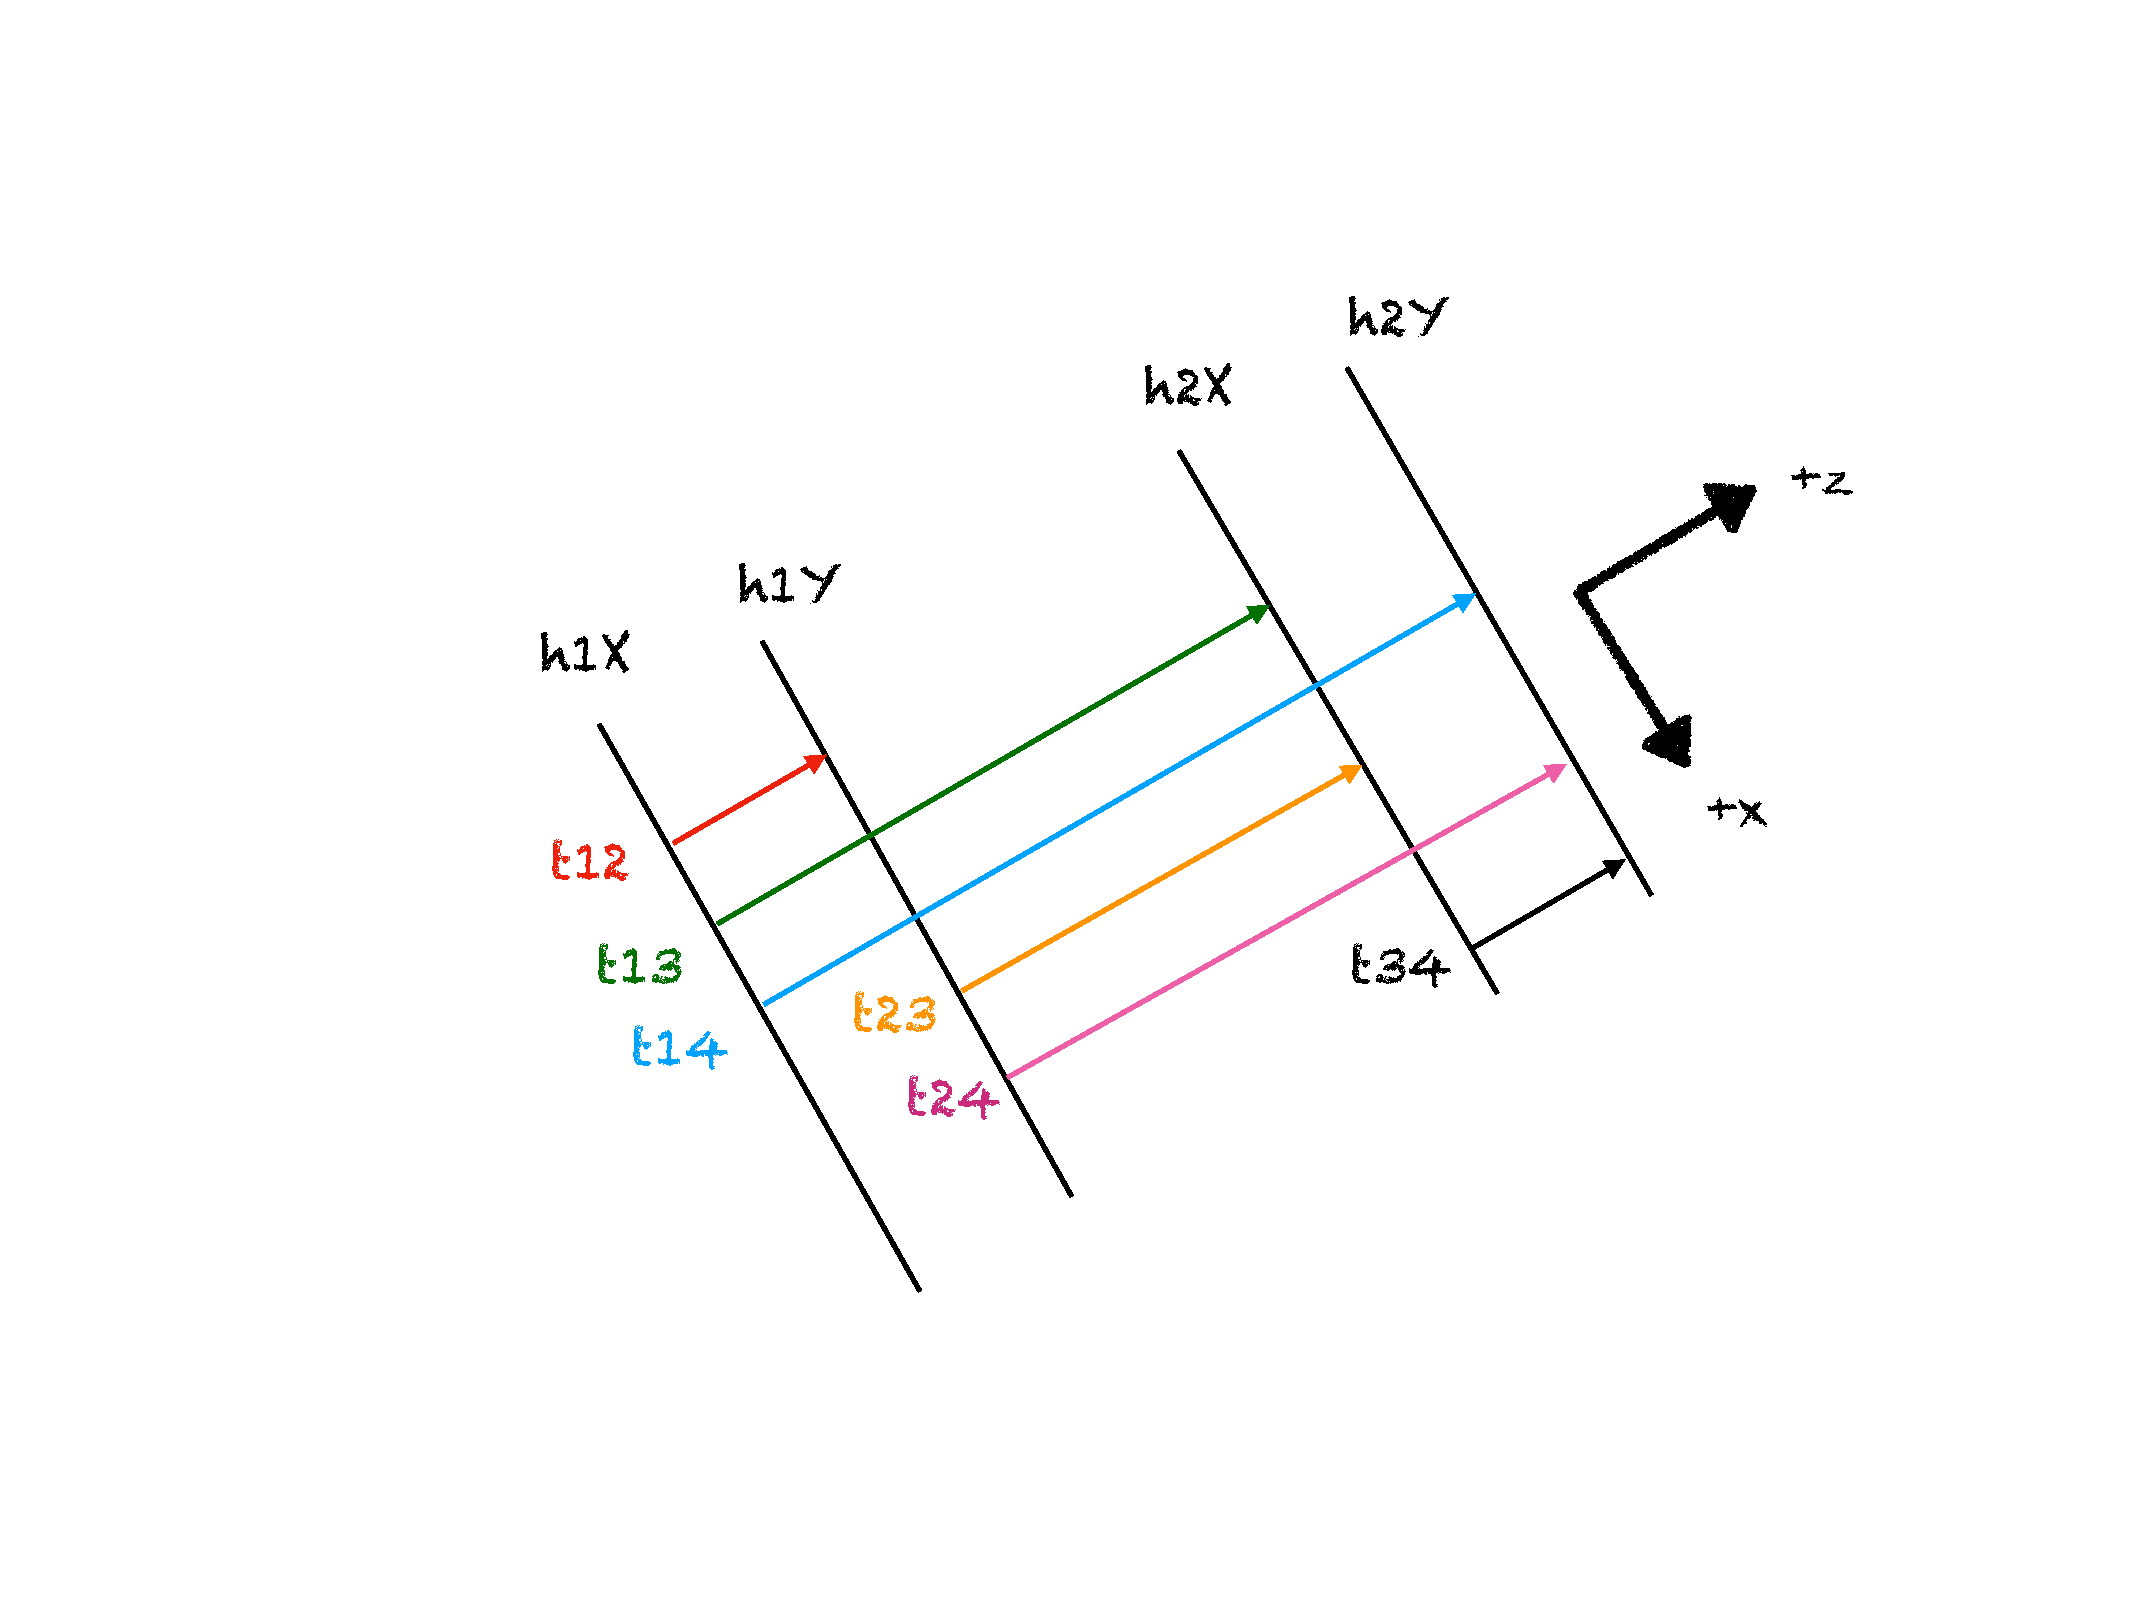
\includegraphics[scale=0.5]{hodo_planes.pdf}
    \caption{Illustration of all possible time difference combinations that are considered in this correction.}
    \label{fig:hod_planes}
\end{figure}
Consider the time difference difference between the $(i,j)$ plane, $t_{ij}$, where the time of the $i$ plane is
given by
\begin{equation}\label{eq:3}
  t_{i} = \frac{T^{(+)}_{TW} + T^{(-)}_{TW} - 2t_{Cable}}{2} 
\end{equation}
From Eq. \ref{eq:3}, $t_{i}$ is the average Time-Walk and cable time corrected TDC time at both ends of the paddle,
and represents the particle arrival time at the paddle. The time difference between any two paddles in the $(i,j)$
planes can be expressed as
\begin{equation} \label{eq:4}
\begin{split}
  &(t_{i} + \lambda_{i}) - (t_{j} + \lambda_{j}) = \frac{D_{ij}}{v_{c}} \\
  &\lambda_{i} - \lambda_{j} = \frac{D_{ij}}{v_{c}} - (t_{i} - t_{j}) \equiv b_{ij}
\end{split}
\end{equation}
where the $\lambda'$s represent small time perturbations that ideally, should \textit{not} be present, but in
reality they are present and need to be accounted for. In front of the $\lambda'$s there are the coefficinets (+1, -1) for
every possible $i,j$ combination. To better understand how to solve the generalized system of linear equations in
Eq. \ref{eq:4}, consider a single event in the HMS in which a single paddle in every plane is hit. The system of six linear equations
corresponding to such event can then be expressed as
\begin{equation} \label{eq:5}
\begin{split}
  &c_{1,1}\lambda_{1} +  c_{1,2}\lambda_{2} + . . . + c_{1,j}\lambda_{j} + . . . + c_{1,52}\lambda_{52} =  b_{12} \\
  &c_{2,1}\lambda_{1} +  c_{2,2}\lambda_{2} + . . . + c_{2,j}\lambda_{j} + . . . + c_{2,52}\lambda_{52} =  b_{13} \\
  &c_{3,1}\lambda_{1} +  c_{3,2}\lambda_{2} + . . . + c_{3,j}\lambda_{j} + . . . + c_{3,52}\lambda_{52} =  b_{14} \\
  &c_{4,1}\lambda_{1} +  c_{4,2}\lambda_{2} + . . . + c_{4,j}\lambda_{j} + . . . + c_{4,52}\lambda_{52} =  b_{23} \\
  &c_{5,1}\lambda_{1} +  c_{5,2}\lambda_{2} + . . . + c_{5,j}\lambda_{j} + . . . + c_{5,52}\lambda_{52} =  b_{24} \\
  &c_{6,1}\lambda_{1} +  c_{6,2}\lambda_{2} + . . . + c_{6,j}\lambda_{j} + . . . + c_{6,52}\lambda_{52} =  b_{34}
\end{split}
\end{equation}
Or in matrix notation,
\begin{align}
\bf{C^{[\lambda]}}\lambda &= \left[\begin{array}{cccccc}
  c_{1,1} & c_{1,2} & \hdots & c_{1,j} & \hdots & c_{1,52} \\
  c_{2,1} & c_{2,2} & \hdots & c_{2,j} & \hdots & \vdots \\
    \vdots & \vdots & \ddots & \hdots & \hdots & \vdots \\
  c_{i,1} & \vdots & c_{i,j} & \ddots & \hdots & \vdots \\
    \vdots & \vdots & \hdots & \hdots & \ddots & c_{5,52} \\
    c_{6,1} & c_{6,2} & \hdots & \hdots & \hdots & c_{6,52} \\
  \end{array}\right]
\begin{bmatrix}
  \lambda_{1}  \\
  \lambda_{2}  \\
  \vdots \\
  \vdots \\
  \lambda_{j} \\
  \vdots \\
  \lambda_{52}
\end{bmatrix} 
= \begin{bmatrix}
  \vspace{5px}
  b_{12}  \\
  \vspace{5px}
  b_{13}  \\
  \vspace{5px}
  b_{14}  \\
  \vspace{5px}
  b_{23}  \\
  \vspace{5px}
  b_{24}  \\
  \vspace{5px}
  b_{34}  \\
\end{bmatrix}
\end{align}
where the left-hand side is a linear combination of the possible perturbative times in all paddles. The index $j$ in $\lambda_{j}$
represents the absolute paddle number, as there are 52 paddles in total in the HMS. The conversion from relative to absolute paddle is as
follows,
\begin{align*}
  &\text{Plane h1X}: \text{Paddles } 1-16,  \lambda_{j}\rightarrow j:1-16 \\
  &\text{Plane h1Y}: \text{Paddles } 1-10,  \lambda_{j}\rightarrow j:17-26 \\
  &\text{Plane h2X}: \text{Paddles } 1-16,  \lambda_{j}\rightarrow j:27-42 \\
  &\text{Plane h2Y}: \text{Paddles } 1-10,  \lambda_{j}\rightarrow j:43-52 
\end{align*}

Assume for this particular event, that paddles
7, 5, 8 and 6 in planes h1X, h1Y, h2X and h2Y respectively, get hit. At this point, all coefficients except those corresponding to the paddles that
fired will be \textit{zero}. The coefficient matrix has the following non-zero terms
\begin{align*}
  &c_{1,7} = 1, c_{1, 21} = -1 \\
  &c_{2,7} = 1, c_{2, 34} = -1 \\
  &c_{3,7} = 1, c_{3, 48} = -1 \\
  &c_{4,21} = 1, c_{4,34} = -1 \\
  &c_{5,21} = 1, c_{5,48} = -1 \\
  &c_{6,34} = 1, c_{6,48} = -1
\end{align*}

\begin{align}
\bf{C^{[\lambda]}} &= \left[\begin{array}{cccccc}
  \hdots & 1 & \hdots & -1 & \hdots & \hdots \\
  \hdots & 1 & \hdots & \hdots & -1 & \hdots \\
  \hdots & 1 & \hdots & \hdots & \hdots & -1  \\
  \hdots & \hdots & 1 & \hdots & -1 & \hdots \\
  \hdots & \hdots & 1 & \hdots & \hdots & -1 \\
  \hdots & \hdots & \hdots & 1 & \hdots & -1 
  \end{array}\right]
\end{align}
\newpage
To simultaneously solve this system of equations for the $\lambda$'s, one event
is not sufficient since not all paddles will fire, and the majority of the $\lambda$'s
will be zero. One needs to sum each of the elements over sufficient events to fill all
coefficients in the matrix and find a solution to all $\lambda$'s as follows,
\begin{align}
\bf{C^{[\lambda]}}\lambda &= \left[\begin{array}{cccccc}
  \sum\limits_{k} c_{1,1} & \sum\limits_{k}c_{1,2} & \hdots & \sum\limits_{k}c_{1,j} & \hdots & \sum\limits_{k}c_{1,52} \\
  \sum\limits_{k}c_{2,1} & \sum\limits_{k}c_{2,2} & \hdots & \sum\limits_{k}c_{2,j} & \hdots & \vdots \\
    \vdots & \vdots & \ddots & \hdots & \hdots & \vdots \\
  \sum\limits_{k}c_{i,1} & \vdots &  \sum\limits_{k}c_{i,j} & \ddots & \hdots & \vdots \\
    \vdots & \vdots & \hdots & \hdots & \ddots &  \sum\limits_{k}c_{5,52} \\
     \sum\limits_{k}c_{6,1} &  \sum\limits_{k}c_{6,2} & \hdots & \hdots & \hdots &  \sum\limits_{k}c_{6,52} \\
  \end{array}\right]
\begin{bmatrix}
  \lambda_{1}  \\
  \lambda_{2}  \\
  \vdots \\
  \vdots \\
  \lambda_{j} \\
  \vdots \\
  \lambda_{52}
\end{bmatrix} 
= \begin{bmatrix}
  \vspace{5px}
   \sum\limits_{k}b_{12}  \\
  \vspace{5px}
   \sum\limits_{k}b_{13}  \\
  \vspace{5px}
   \sum\limits_{k}b_{14}  \\
  \vspace{5px}
   \sum\limits_{k}b_{23}  \\
  \vspace{5px}
   \sum\limits_{k}b_{24}  \\
  \vspace{5px}
   \sum\limits_{k}b_{34}  \\
\end{bmatrix}
\end{align}
There are various methods to solve a system of linear equations. Some which might
be more numerically stable than others. For this specific case, Single-Value Decomposition (SVD)
method was used. 
% j=7, 21, 34, 48 

\item Propagation Time Corrections, $t_{prop.}$: This correction accounts for the propagation
  time across both ends of the scintillator paddle from the particle hit location. The corrections is
  done in the Hall C Analyzer, \textit{hcana}. Some of the geometrical parameters that are used are shown
  in Figure \ref{fig:propTime}. \\
  \begin{figure}[H]
    \captionsetup{justification=raggedright,singlelinecheck=false}
    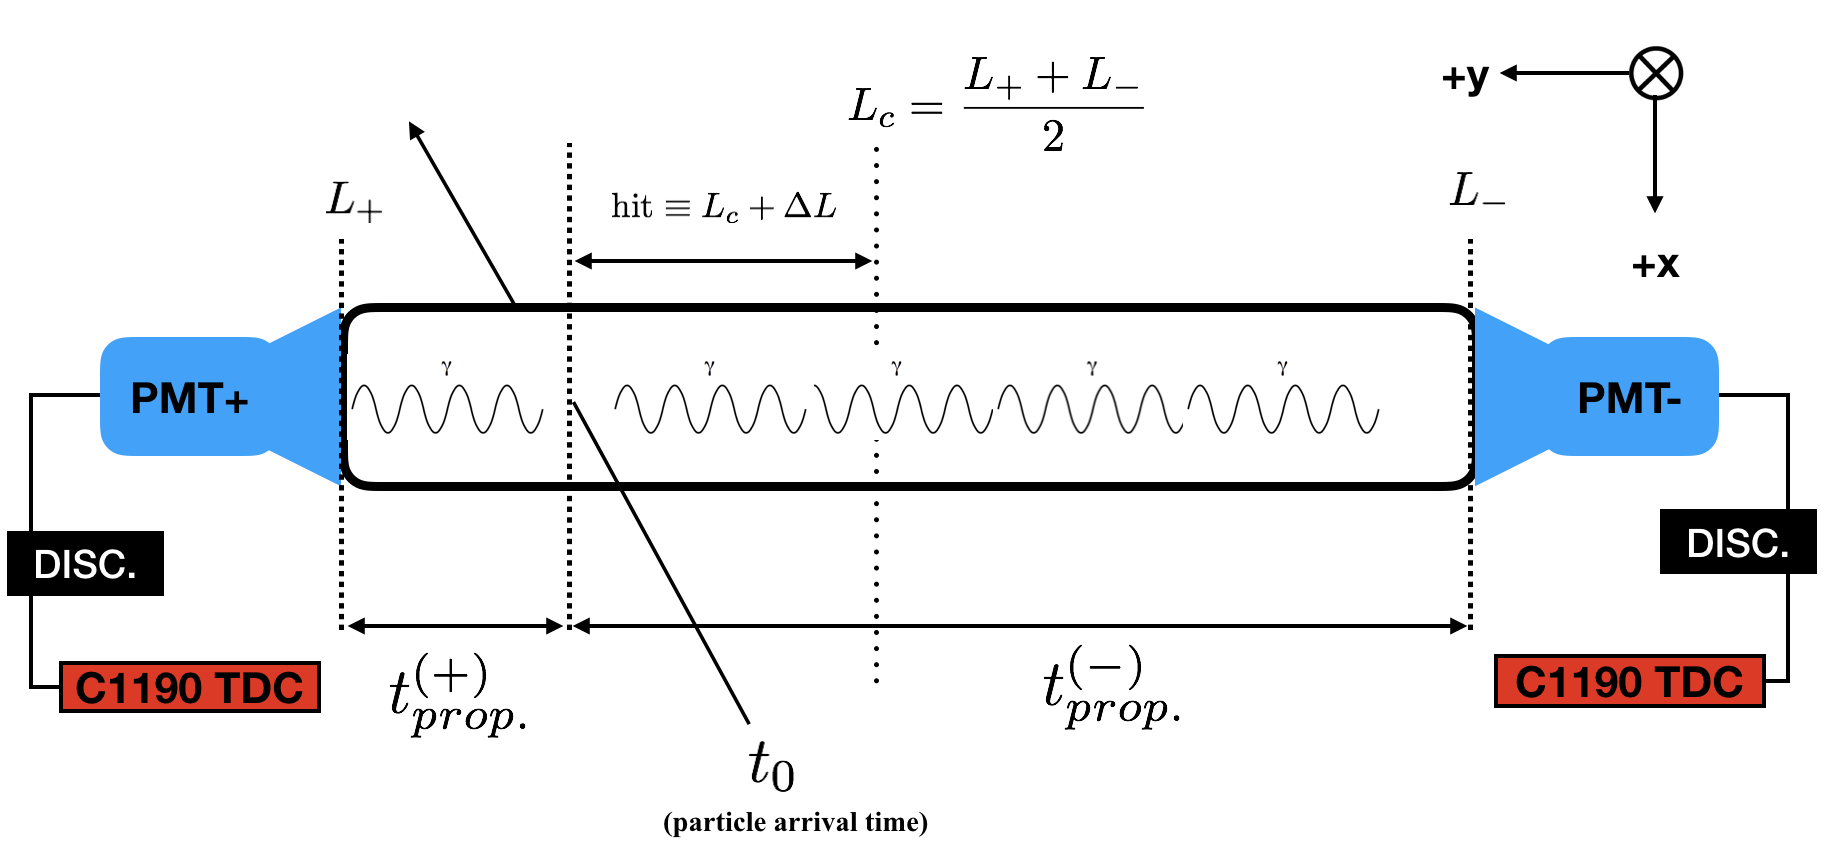
\includegraphics[scale=0.48]{propTime_Corr.png}
    \caption{Scintillator paddle illustrating how to apply the propagation time corrections.}
    \label{fig:propTime}
  \end{figure}
  To derive how this correction is done in hcana, let the time-walk and cable length corrected time be
  defined as
  \begin{equation}
    t^{\pm}_{Corr.} = t_{0} + t^{\pm}_{prop.}
  \end{equation}
  The path length from the center of the paddle to the hit can then be defined as
    \begin{align}
      \Delta L &= \frac{1}{2}(t^{(-)}_{Corr.} - t^{(+)}_{Corr.})v_{p} =  \frac{1}{2}(t^{(-)}_{prop.} - t^{(+)}_{prop.})v_{p}
    \end{align}
    The equations used in hcana are
    \begin{align}\label{eq:11}
      t^{(+)}_{Corr.} = t^{(+)}_{Corr.} - (L_{+} - hit)\frac{1}{v_{p}}, \text{ where } t^{(+)}_{prop.}\equiv(L_{+} - hit)\frac{1}{v_{p}} \nonumber \\
      t^{(-)}_{Corr.} = t^{(-)}_{Corr.} - (hit - L_{-})\frac{1}{v_{p}}, \text{ where } t^{(-)}_{prop.}\equiv(hit - L_{-})\frac{1}{v_{p}}       
    \end{align}
    Substituting the definitions from Figure \ref{fig:propTime}  into Eq.\ref{eq:11}, after some algebra, one is able to prove that
    \begin{equation}
      t_{avgCorr} = \frac{1}{2}( t^{(+)}_{Corr.} +  t^{(-)}_{Corr.}) = \frac{1}{2} (t^{(+)}_{TWC_{orr.}} +  t^{(-)}_{TW_{Corr.}})
    \end{equation}
    where the propagation time has been corrected for.
\end{itemize}

\renewcommand{\labelitemi}{$\blacksquare$}


\section{Hodoscope Calibration Procedure}
In this section I will discuss the procedure to perform the hodoscopes calibration
using the new method.
\begin{itemize}
\item Set the flag \texttt{h(p)tofusinginvadc = 0} to NOT use the hodo parameters from the
  previous hodoscope calibration procedure. This flag is found on \texttt{hallc\_replay/PARAM/H(S)MS/HODO/} directory.
\item Replay the raw data file, typically 1-2 M events is required for a good fit to be done.   
\item In the directory \texttt{hallc\_replay/CALIBRATION/(s)hms\_hodo\_calib/}, run the following code:
  \subitem $\Diamond$ {\texttt{root -l ''timeWalkHistos.C(<run\_num>)''} \\
  This script takes as input the ROOTfile replayed and creates another ROOTfile with histogram
  objects that are used to perform the time-walk correction.}
\item To do the time-walk corrections, run the following code:
  \subitem $\Diamond$ {\texttt{root -l ''timeWalkCalib.C(<run\_num>)''}} \\
  This script takes as input the ROOTfile containing the histogram objects produced by the previous
  script.  A parameter file containing the time-walk parameters will be produced at 
  \subitem $\Diamond$ {\texttt{hallc\_replay/PARAM/(S)HMS/HODO/(p)hhodo\_TWcalib\_runNUM.param}}
  This parameter file name has to be manually changed to exclude the run number, since hcana reads in the parameter file as
  \texttt{(p)hhodo\_TWcalib.param} .
\item Replay the raw data file, once again (1 - 2 M events), with the updated time-walk parameters.
\item In the hodoscopoe calibration directory, run the following code:
  \subitem $\Diamond$ {\texttt{root -l fitHodoCalib.C}}
  The first part of this script performs a linear fit on the time-walk corrected time vs. hodoscope track
  to determine the propagation velocity and the cable time difference across each paddle. The second part of
  this code solves a matrix equation for the $\lambda$ parameters mentioned in the previous section.
  A parameter file containing the time-walk parameters will be produced at
  \subitem $\Diamond$ {\texttt{hallc\_replay/PARAM/(S)HMS/HODO/(p)hhodo\_Vpcalib\_runNUM.param}} \\
  This parameter file name has to be manually changed to exclude the run number, since hcana reads in the parameter file as
  \texttt{(p)hhodo\_Vpcalib.param} .
\item {Replay the raw data one last time, and check the hodoscope beta distribution. You may have to apply a calorimeter cut (for example, \texttt{(P)H.cal.etracknorm>0.7})}
  A good calibration should have the beta centered at unity. (See Figure \ref{fig:beta})
\end{itemize}
\begin{figure}[H]
    \captionsetup{justification=raggedright,singlelinecheck=false}
    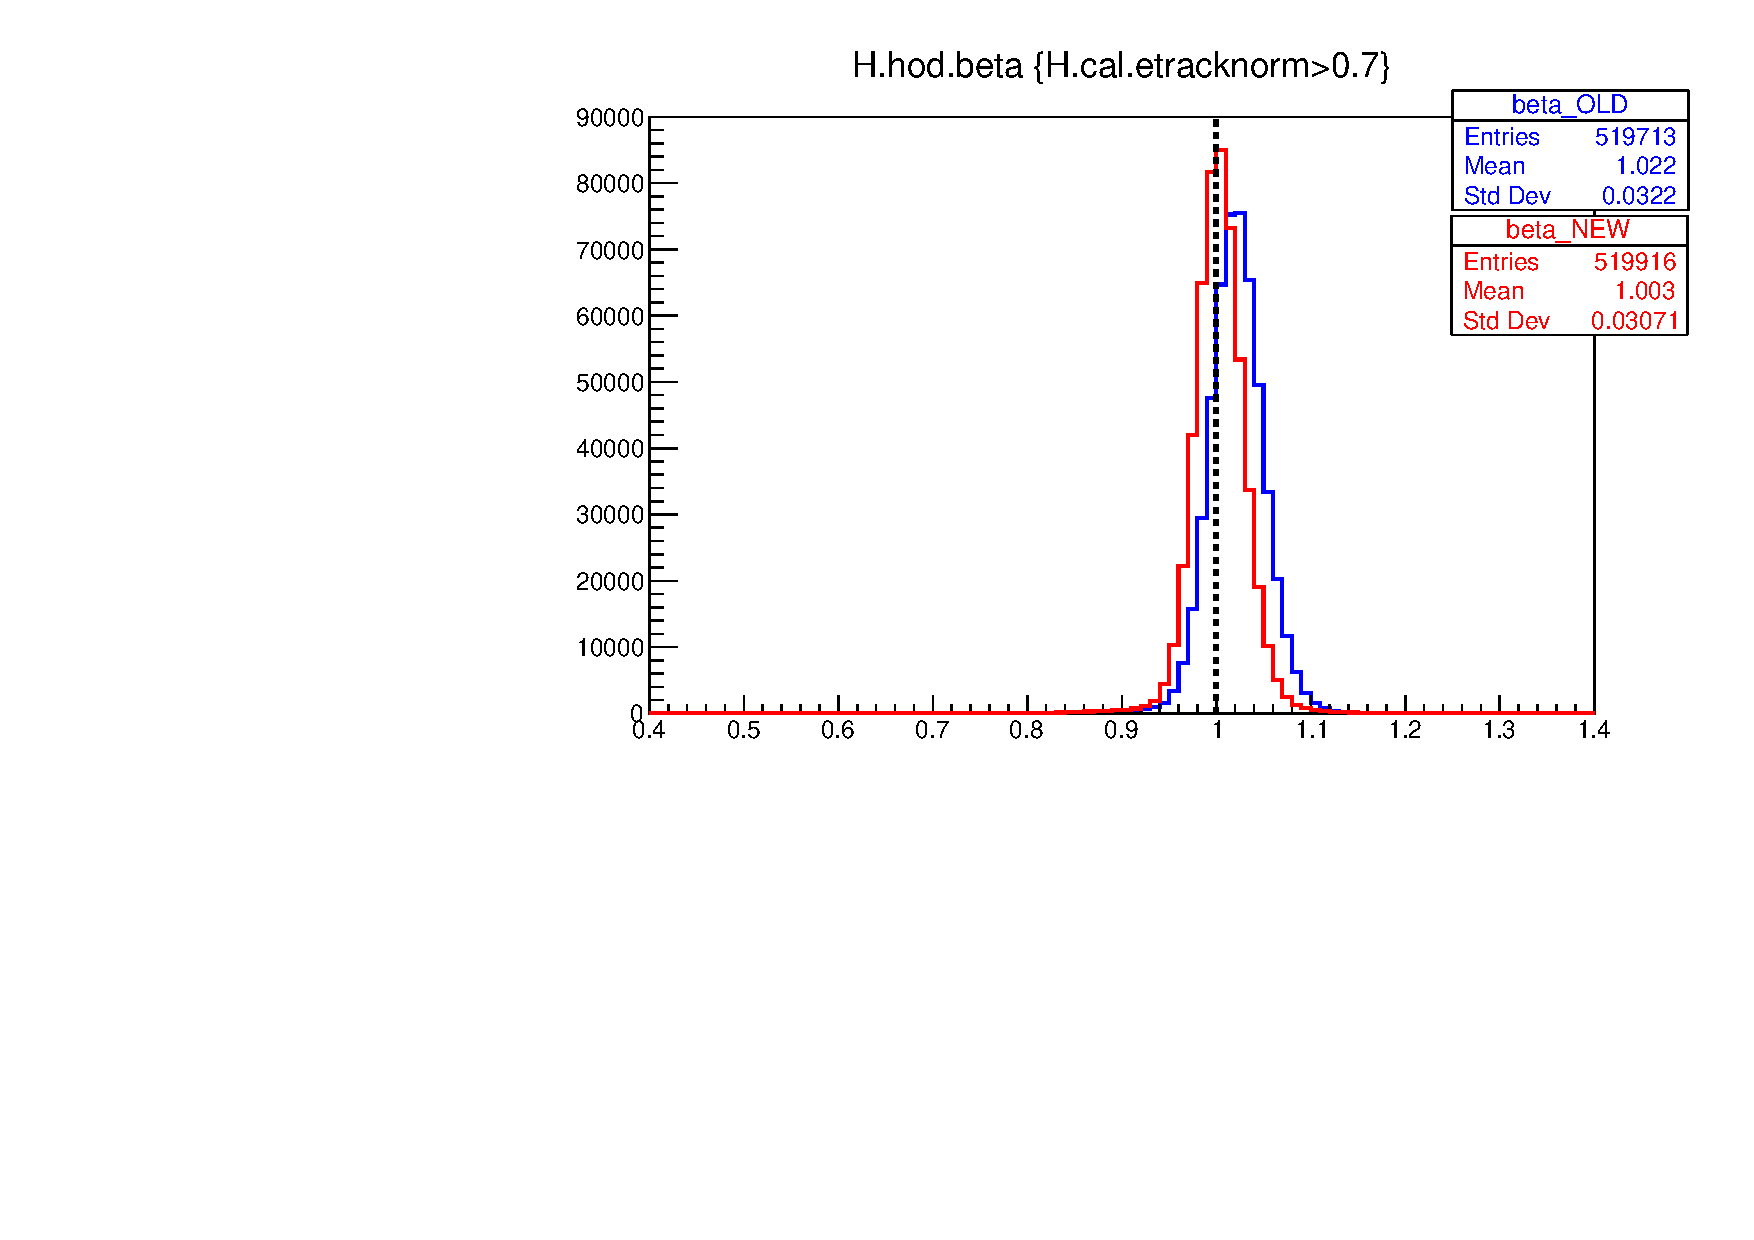
\includegraphics[scale=0.7]{hms_betaCompare.pdf}
    \caption{Comparison between HMS $\beta$ distributions using the original and new calibration procedure.}
    \label{fig:beta}
\end{figure}
%HHODO_vPcalib.param, fitHodoCalib.C


% --------------------------------------------------------------
%     You don't have to mess with anything below this line.
% --------------------------------------------------------------
 
\end{document}
